\PassOptionsToPackage{unicode=true}{hyperref} % options for packages loaded elsewhere
\PassOptionsToPackage{hyphens}{url}
%
\documentclass[ignorenonframetext,]{beamer}
\usepackage{pgfpages}
\setbeamertemplate{caption}[numbered]
\setbeamertemplate{caption label separator}{: }
\setbeamercolor{caption name}{fg=normal text.fg}
\beamertemplatenavigationsymbolsempty
% Prevent slide breaks in the middle of a paragraph:
\widowpenalties 1 10000
\raggedbottom
\setbeamertemplate{part page}{
\centering
\begin{beamercolorbox}[sep=16pt,center]{part title}
  \usebeamerfont{part title}\insertpart\par
\end{beamercolorbox}
}
\setbeamertemplate{section page}{
\centering
\begin{beamercolorbox}[sep=12pt,center]{part title}
  \usebeamerfont{section title}\insertsection\par
\end{beamercolorbox}
}
\setbeamertemplate{subsection page}{
\centering
\begin{beamercolorbox}[sep=8pt,center]{part title}
  \usebeamerfont{subsection title}\insertsubsection\par
\end{beamercolorbox}
}
\AtBeginPart{
  \frame{\partpage}
}
\AtBeginSection{
  \ifbibliography
  \else
    \frame{\sectionpage}
  \fi
}
\AtBeginSubsection{
  \frame{\subsectionpage}
}
\usepackage{lmodern}
\usepackage{amssymb,amsmath}
\usepackage{ifxetex,ifluatex}
\usepackage{fixltx2e} % provides \textsubscript
\ifnum 0\ifxetex 1\fi\ifluatex 1\fi=0 % if pdftex
  \usepackage[T1]{fontenc}
  \usepackage[utf8]{inputenc}
  \usepackage{textcomp} % provides euro and other symbols
\else % if luatex or xelatex
  \usepackage{unicode-math}
  \defaultfontfeatures{Ligatures=TeX,Scale=MatchLowercase}
\fi
% use upquote if available, for straight quotes in verbatim environments
\IfFileExists{upquote.sty}{\usepackage{upquote}}{}
% use microtype if available
\IfFileExists{microtype.sty}{%
\usepackage[]{microtype}
\UseMicrotypeSet[protrusion]{basicmath} % disable protrusion for tt fonts
}{}
\IfFileExists{parskip.sty}{%
\usepackage{parskip}
}{% else
\setlength{\parindent}{0pt}
\setlength{\parskip}{6pt plus 2pt minus 1pt}
}
\usepackage{hyperref}
\hypersetup{
            pdftitle={Méthodes de Monte Carlo et inférence bayésienne},
            pdfauthor={Pierre Gloaguen},
            pdfborder={0 0 0},
            breaklinks=true}
\urlstyle{same}  % don't use monospace font for urls
\newif\ifbibliography
\setlength{\emergencystretch}{3em}  % prevent overfull lines
\providecommand{\tightlist}{%
  \setlength{\itemsep}{0pt}\setlength{\parskip}{0pt}}
\setcounter{secnumdepth}{0}

% set default figure placement to htbp
\makeatletter
\def\fps@figure{htbp}
\makeatother


\title{Méthodes de Monte Carlo et inférence bayésienne}
\providecommand{\subtitle}[1]{}
\subtitle{Introduction}
\author{Pierre Gloaguen}
\date{\href{mailto:pierre.gloaguen@agroparistech.fr}{\nolinkurl{pierre.gloaguen@agroparistech.fr}}}

\begin{document}
\frame{\titlepage}

\begin{frame}{Déroulé du cours}
\protect\hypertarget{duxe9rouluxe9-du-cours}{}

\begin{itemize}
\tightlist
\item
  7 séances de 3h;
\item
  Chaque début de séance consacré aux questions et à la présentation du
  cours;
\item
  TD en autonomie ensuite (avec réponse aux questions);
\item
  Evaluation en contrôle continu (exercices à rendre);
\end{itemize}

\end{frame}

\begin{frame}[fragile]{Objectifs de cette 1ère séance}
\protect\hypertarget{objectifs-de-cette-1uxe8re-suxe9ance}{}

\begin{itemize}
\tightlist
\item
  Introduction et motivation du sujet du cours;
\item
  Principe des méthodes de Monte Carlo;
\item
  Premiers exercices et implémentation sous \texttt{R}.
\end{itemize}

\end{frame}

\hypertarget{introduction-et-motivations}{%
\section{Introduction et
motivations}\label{introduction-et-motivations}}

\begin{frame}{Modèlisation statistique}
\protect\hypertarget{moduxe8lisation-statistique}{}

\begin{itemize}
\tightlist
\item
  Formulation probabiliste d'un problème:

  \begin{itemize}
  \tightlist
  \item
    \emph{On suppose que les données sont les réalisations de variables
    aléatoires telles que \(\dots\)};
  \end{itemize}
\item
  Quantification de l'incertitude:

  \begin{itemize}
  \tightlist
  \item
    \emph{d'après le modèle posé, la probabilité que tel événement
    arrive est de \(\dots\)};
  \end{itemize}
\item
  Recours permanent au \textbf{calcul de probabilités};
\end{itemize}

\end{frame}

\begin{frame}{Exemple immédiat}
\protect\hypertarget{exemple-immuxe9diat}{}

\begin{itemize}
\tightlist
\item
  Test d'hypothèse: On veut tester une hypothèse \(H_0\) contre une
  hypothèse \(H_1\)

  \begin{itemize}
  \tightlist
  \item
    \emph{Ex: Comparaison de moyennes de deux échantillons Gaussiens};
  \end{itemize}
\item
  On construit une statistique de test \(T\);
\item
  Décision binaire, pour un risque de première espèce \(\alpha\), on
  définit un zone de rejet \(\mathcal{R}\), telle que
\end{itemize}

\[\mathbb{P}_{H_0}\left(T \in \mathcal{R}\right) = \alpha\]

\pause

\textbf{Rappel:}
\[\mathbb{P}_{H_0}\left(T \in \mathcal{R}\right) = \mathbb{E}_{H_0}\left[\mathbf{1}_{T\in \mathcal{R}}\right]\]

\begin{itemize}
\tightlist
\item
  On doit donc être capable d'évaluer une espérance (ici, la probabilité
  d'évènements) sous \(H_0\) pour construire notre test.
\end{itemize}

\end{frame}

\begin{frame}{Exemple de modèle statistique: Biomasse d'une population
de poisson}
\protect\hypertarget{exemple-de-moduxe8le-statistique-biomasse-dune-population-de-poisson}{}

\begin{tabular}{cc}
\multicolumn{2}{c}{\textbf{Ce qu'on connaît}} \\ 
{\color{red} Captures $C$} & {\color{blue} Observations scientifiques $Y$}\\
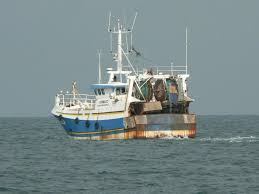
\includegraphics[height = 3cm, width = 0.4\textwidth]{figures/chalutier} & 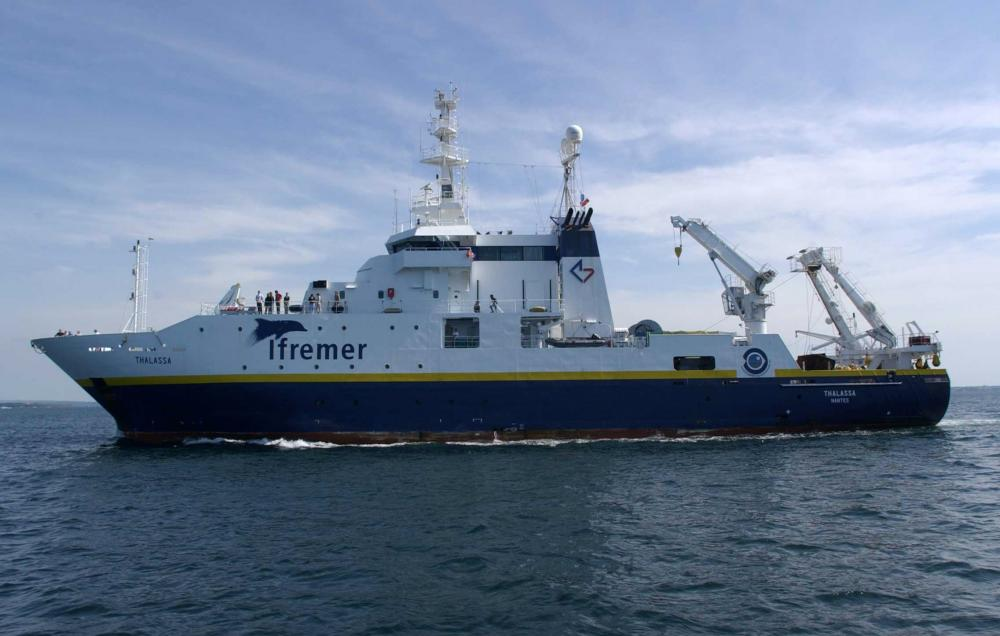
\includegraphics[height = 3cm, width = 0.4\textwidth]{figures/thalassa}\\
\multicolumn{2}{c}{\textbf{Quantité d'intérêt}}\\ 
\multicolumn{2}{c}{Biomasse de poisson $X$}  \\ 
\multicolumn{2}{c}{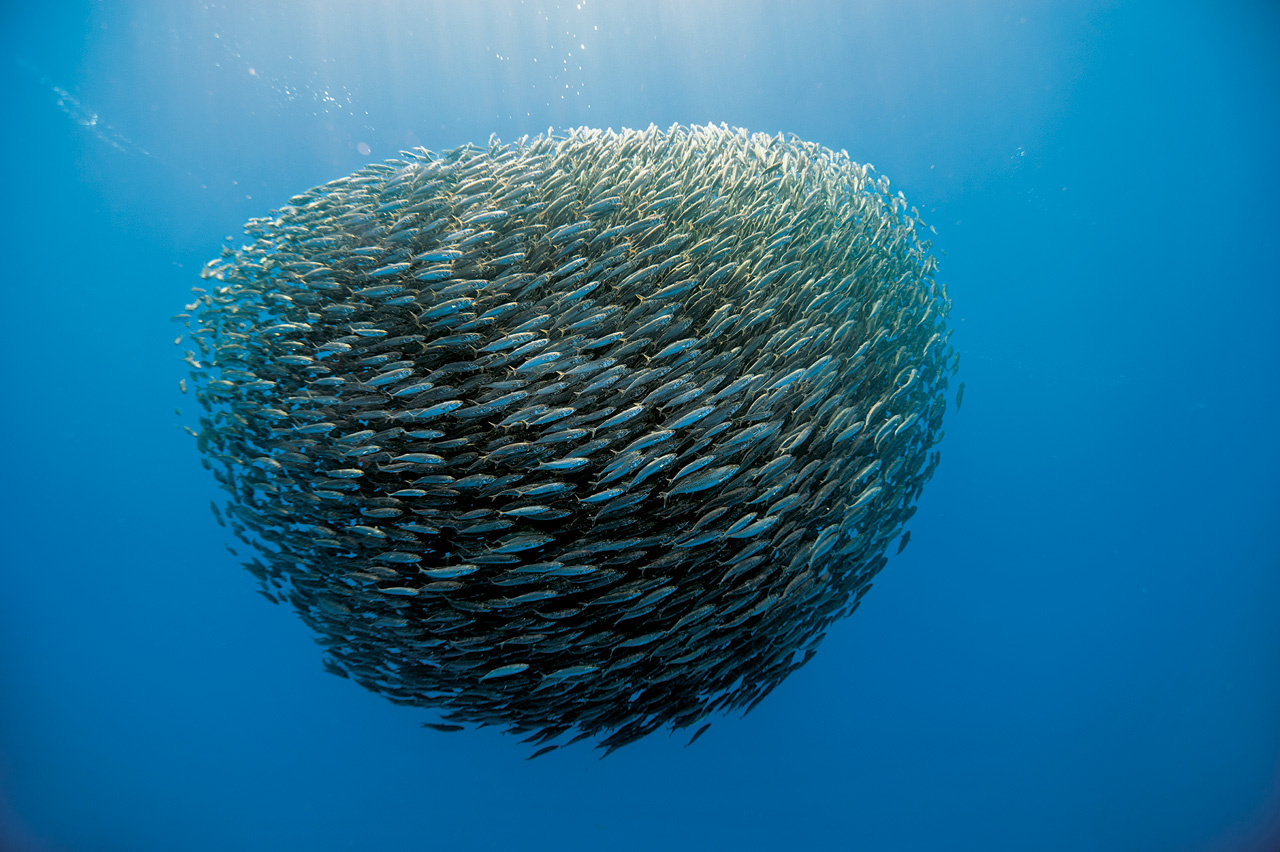
\includegraphics[width = 0.4\textwidth]{figures/poissons}}
\end{tabular}

\textbackslash{}end\{frame\}

\end{frame}

\begin{frame}{Modèle probabiliste d'observation de la dynamique de
population}
\protect\hypertarget{moduxe8le-probabiliste-dobservation-de-la-dynamique-de-population}{}

\begin{align*}
X_{t+1} &= \left( X_t + {\color{purple}r} X_t\left(1- \frac{X_t}{\color{purple}K}\right) - {\color{red} C_t} \right) \exp(\varepsilon_{t + 1}), \text{ Biomasse cachée}\\
{\color{blue} Y_t}\vert X_t &= {\color{purple}q} X_t \exp(\nu_{t}),~ {\color{red} C_t} \text{ Observations}\\
\varepsilon_t& \overset{i.i.d}{\sim}\mathcal{N}\left(-{\color{purple} \sigma}^2 / 2, {\color{purple}\sigma}^2\right),~~\nu_t\overset{i.i.d}{\sim}\mathcal{N}\left(-{\color{purple}\sigma}_\text{obs}^2 / 2, {\color{purple} \sigma}_\text{obs}^2\right).
\end{align*}

\begin{itemize}
\tightlist
\item
  \(X_t\): Biomasse à l'année \(t\) (non observée);
\item
  \(Y_t\): Abundance observée à l'année \(t\);
\item
  \(C_t\): Captures à l'année \(t\);
\item
  \(K\): Capacité d'accueil du milieu (paramètre);
\item
  \(r\): Taux de croissance de la population (paramètre);
\item
  \(\sigma, \sigma_\text{obs}\): Paramètres de l'aléa;
\item
  \(q\): Détectabilité (paramètre);
\end{itemize}

\end{frame}

\begin{frame}{Questions classiques d'inférence}
\protect\hypertarget{questions-classiques-dinfuxe9rence}{}

\pause

\begin{itemize}
\tightlist
\item
  Pour un tel modèle, étant donnée une population initiale \(X_0\),
  quelle est la moyenne attendue du nombre de poissons au bout de 10 ans
  si on se fixe une quantité de captures?\pause

  \begin{itemize}
  \tightlist
  \item
    \(\mathbb{E}\left[X_{10} \vert X_0 \right]\)?\pause
  \end{itemize}
\item
  Etant données des observations sur 10 années, et en supposant tous les
  paramètres connus, que puis je dire sur la quantité de poissons qu'il
  y avait durant ces 10 ans? \pause

  \begin{itemize}
  \tightlist
  \item
    \(\mathbb{E}\left[X_{0:10} \vert Y_{0:10} \right]\)? \pause
  \end{itemize}
\item
  Etant données des observations, que puis je dire sur la valeur des
  paramètres de dynamique de population?\pause

  \begin{itemize}
  \tightlist
  \item
    Inférence des paramètres:
  \item
    Méthode des moments (nécessite un calcul d'espérance);\pause
  \item
    Méthode du maximum de vraisemblance (nécessite ici un calcul
    d'espérance);\pause
  \item
    Estimateur Bayésien: Nécessite un calcul d'espérance. \pause
  \end{itemize}
\end{itemize}

Ces espérances n'ont, en général, pas d'expressions directes!

\end{frame}

\begin{frame}{Méthodes de Monte Carlo}
\protect\hypertarget{muxe9thodes-de-monte-carlo}{}

\pause

\begin{itemize}
\tightlist
\item
  \textbf{But:} Approcher des espérances (intégrales) en utilisant des
  simulations probabilistes; \pause
\item
  \textbf{Idée:} La loi des grands nombres! La moyenne empirique d'une
  variable aléatoire va tendre, si on répète l'expérience, vers la
  moyenne théorique.
\end{itemize}

\end{frame}

\begin{frame}{Exemple}
\protect\hypertarget{exemple}{}

On dispose d'un dé à 6 faces et seulement de ce dé. Comment peut on
essayer de savoir s'il est biaisé?

\begin{itemize}
\tightlist
\item
  Si on lance le dé suffisament de fois, on obtient une
  information;\pause
\item
  Combien de fois faut il lancer le dé pour avoir une idée
  précise?\pause
\item
  À quel point peut être confiant en notre réponse?\pause
\item
  Encore faut il savoir lancer le dé!
\end{itemize}

\end{frame}

\begin{frame}{Programme du cours}
\protect\hypertarget{programme-du-cours}{}

\begin{itemize}
\tightlist
\item
  Présentation formelle des méthodes de Monte Carlo pour le calcul
  d'intégrales;
\item
  Application directe en statistique classique (évaluation d'une
  probabilité, aide à la décision);\pause
\item
  Comment peut on simuler des variables aléatoires génériques (avec un
  ordinateur)?\pause
\item
  Une méthode d'inférence dépendante de la simulation: l'inférence
  bayésienne;\pause
\item
  Une extension nécessaire, les Méthodes de Monte Carlo par chaîne de
  Markov (MCMC).
\end{itemize}

\end{frame}

\begin{frame}[fragile]{Prérequis}
\protect\hypertarget{pruxe9requis}{}

\begin{itemize}
\tightlist
\item
  Résulats statistiques asymptotiques:

  \begin{itemize}
  \tightlist
  \item
    Loi des grands nombres, théorème central limite, lemme de Slutsky,
    Delta méthode.
  \end{itemize}
\item
  Chaînes de Markov:

  \begin{itemize}
  \tightlist
  \item
    Loi de transition, irréductibilité, périodicité, mesure invariante
    \(\dots\)
  \end{itemize}
\item
  Logiciel \texttt{R}

  \begin{itemize}
  \tightlist
  \item
    Logiciel \texttt{R} installé ainsi que l'IDE \texttt{Rstudio}.
  \item
    Connaissance minimale du langage (boucles, fonctions, graphiques de
    base\ldots{}).
  \end{itemize}
\end{itemize}

\end{frame}

\end{document}
